\section{Isogeometric analysis}
\label{sec:iga}
IGA is basically an extension of the FEM using either B-splines or non-uniform rational B-splines (NURBS) as basis functions not only representing the geometry, but also the solution space. Being introduced in 2005 by Hughes et al.~\cite{Hughes2005iac}, followed by the book~\cite{Cottrell2009iat} in 2009, IGA tries to bridge the gap between finite element analysis and computer aided design (CAD) tools. The important feature of IGA is that it uses the same basis as CAD software for describing the given geometry, and thus exact representation of the model is possible. It is therefore natural to include a section considering this basis in the beginning before we set up the IGA for the problem at hand.

The isogeometric framework is illustrated in~\Cref{Fig:wineGlass}, where a wine glass is used as an example. Products are often designed in CAD software which enables rendering (or image synthesis) functionality for a photorealistic view of the product. Before producing a visually satisfactory product it is often of interest to do some analysis to check whether or not the product serves its purpose. For decades the finite element method (FEM) has been a crucial framework where this analysis has been obtained. FEM requires an analysis suitable discretization of the model before analysis can be performed. The isogeometric analysis (IGA) framework tries to avoid this discretization step as it uses the parametrization directly from the CAD model. A significant amount of time has traditionally been needed in this step ($\sim 80\%$), and so the potential of the isogeometric framework is for this reason alone very intriguing. In the realm of local refinement, it should be mentioned that creating an analysis suitable model is a hot research topic also in the IGA community~\cite{Bazilevs2010iau,Scott2011tsa,Scott2012lro,Scott2013ibe,Evans2015hts,Sangalli2016uss,Toshniwal2017scs}. The IGA framework may also be used in the post processing step where the visualization is computed using the same NURBS basis from analysis~\cite{Stahl2017ppa}. Finally, it turns out that the spline basis functions are particularly suited to solve elliptical problems~\cite{BeiraodaVeiga2011sef,BeiraodaVeiga2014mao}. This effect is arguably the main motivator for using IGA in this work as numerical dispersion and dissipation errors are reduced in wave propagation problems~\cite{Cottrell2007sor,Dede2015ind,Wen2018aqb,Pegolotti2019iao}. One can then conclude that IGA is particularly well suited to solve acoustic scattering problems.

\begin{figure}
	\centering    
	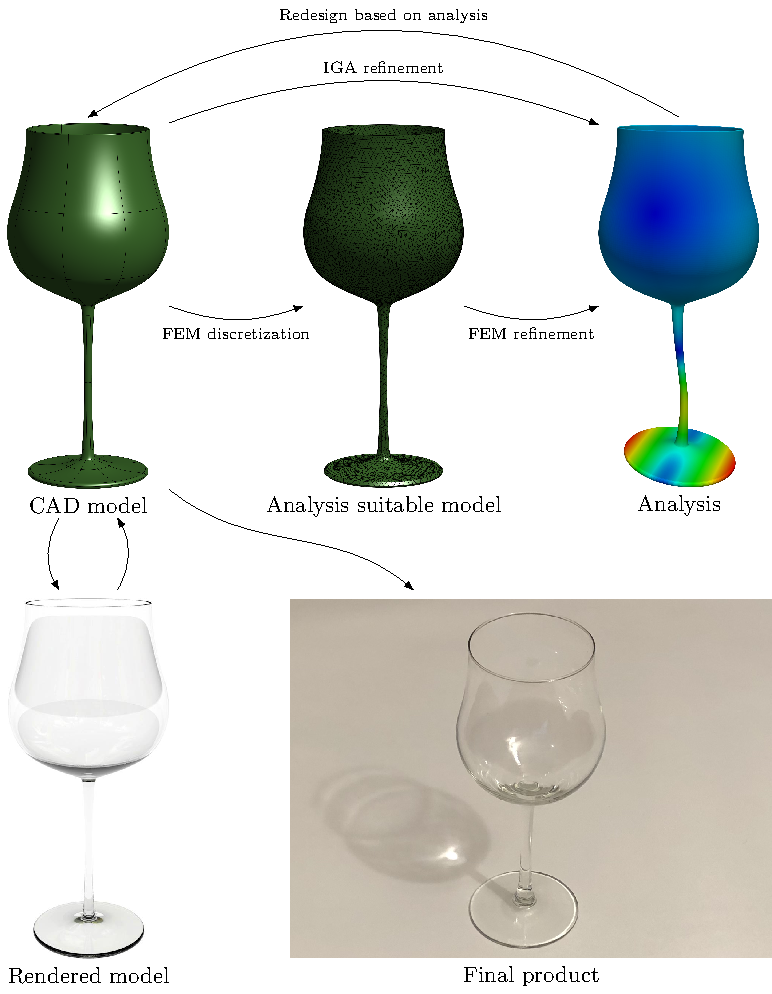
\includegraphics{wineGlass}
	\caption{\textbf{The isogeometric framework}: Isogeometric analysis (IGA) avoids the creation of an analysis suitable discretization step of the finite element method (FEM) as it uses the discretization given by the computer aided design (CAD) system.}
	\label{Fig:wineGlass}
\end{figure}

The classical $\check{p}$-refinement and $h$-refinement are often obtained for more accurate solutions in FEA. IGA comes with an additional refinement feature called the $\check{k}$-refinement with not only an increase in polynomial order, but also the continuity. This is the beauty of IGA as it allows control of the continuity in the discretization spaces. The mathematical potential of the $\check{k}$-refinement is presented in~\cite{BeiraodaVeiga2011sef}, and the application of this technique will be illustrated in paper II and paper III.

Since IGAs conception in 2005, it has obtained an impressive growth in terms of published articles, citations and active researchers in the field. IGA has excelled in a number of applications including continuum damage models~\cite{Verhoosel2011aia}, blood flow~\cite{Bazilevs2006ifi,Zhang2007psv,Morganti2015psi}, free surface flow~\cite{Akkerman2011iao}, wind energy~\cite{Hsu2011hpc,Bazilevs2012ifi}, fracture mechanics~\cite{Borden2012apf,Borden2014aho,Moutsanidis2018hpf}, topology optimization~\cite{Dede2012iaf}, shape optimization~\cite{Manh2011iso,Kiendl2014iso}, shell theory~\cite{Benson2010isa}, contact problems~\cite{Dittmann2014iaa,Temizer2011cti}, structural vibrations~\cite{Cottrell2006iao}, immersed boundary methods~\cite{Schillinger2012aid}, sliding interfaces~\cite{Bazilevs2008nbi}, and phase-field modeling~\cite{Gomez2008iao}. The academic interest of IGA has so far been a huge success, and it remains to see when the industry fully incorporates this progress into modeling software. Classical finite element technologies are deeply rooted into comprehensive software, but we can already see several major software companies showing interest (i.e. Abaqus~\cite{Lai2017icw}).	

\subsection{B-splines}
\renewcommand{\Xi}{{\vec{t}}}
The NURBS basis is constructed using B-splines. Therefore, an understanding of B-splines is crucial to understanding NURBS. Let $\check{p}$ be the polynomial order\footnote{The usage of a check sign above the polynomial order $p$ is to avoid ambiguity between the polynomial order and the scattered pressure.}, let $n$ be the number of basis functions and define a \textit{knot vector} $\Xi = \{\xi_1,\xi_2,\dots,\xi_{n+\check{p}+1}\}$ to be an ordered vector with non-decreasing elements, called \textit{knots}. Then, the $n$ B-splines, $\left\{B_{i,\check{p},\Xi}\right\}_{i\in [1,n]}$, are recursively defined by
\begin{equation*}
	B_{i,\check{p},\Xi}(\xi) = \frac{\xi-\xi_i}{\xi_{i+\check{p}}-\xi_i}B_{i,\check{p}-1,\Xi}(\xi)+\frac{\xi_{i+\check{p}+1} - \xi}{\xi_{i+\check{p}+1} -\xi_{i+1}}B_{i+1,\check{p}-1,\Xi}(\xi)
\end{equation*}
starting with
\begin{equation}\label{Eq:orderOneBspline}
	B_{i,0,\Xi}(\xi)=\begin{cases}
		1 & \text{if } \xi_i\leq \xi < \xi_{i+1}\\
		0 & \text{otherwise.}
	\end{cases}
\end{equation}
This formula is referred to as Cox-de Boor formula, and the derivative of a B-spline may be computed by
\begin{equation}\label{Eq:derivBspline}
	\frac{\diff}{\diff\xi} B_{i,\check{p},\Xi}(\xi) = \frac{\check{p}}{\xi_{i+\check{p}}-\xi_{i}}B_{i,\check{p}-1,\Xi}(\xi)-\frac{\check{p}}{\xi_{i+\check{p}+1}-\xi_{i+1}}B_{i+1,\check{p}-1,\Xi}(\xi).
\end{equation} 
Throughout this work, we shall use \textit{open knot vectors} (in order to easily handle boundary conditions). That is, the first and last element in the vector are repeated $\check{p}+1$ times. Moreover, a knot is said to have \textit{multiplicity} $m$ if it is repeated $m$ times in $\Xi$.

Some important properties of B-splines are given by the following (for proof, cf.~\cite{Lyche2008smd}).
\label{List:properties}
\begin{enumerate}
	\item $B_{i,\check{p},\Xi}$ are piecewise polynomials.
	\item $B_{i,\check{p},\Xi}$ depends only on the knots $\xi_i,\xi_{i+1},\dots,\xi_{i+\check{p}+1}$.
	\item In general $B_{i,\check{p},\Xi}(\xi)\geq 0$, and if $\xi\not\in [\xi_i, \xi_{i+\check{p}+1})$ then $B_{i,\check{p},\Xi}(\xi) = 0$.
	\item If $\xi\in [\xi_j, \xi_{j+1})$ then $B_{i,\check{p},\Xi}(\xi) = 0$ if $i < j-\check{p}$ or $i>j$.
	\item If $\xi\in (\xi_i,\xi_{i+\check{p}+1})$ then $B_{i,\check{p},\Xi}(\xi) > 0$.
	\item If $\tilde{\xi} = \xi_{j+1} = \dots = \xi_{j+\check{p}} < \xi_{j+\check{p}+1}$ then $B_{i,\check{p},\Xi}\Big(\tilde{\xi}\Big) = \delta_{ij}$.
	\item If a knot $\tilde{\xi}\in \{\xi_i,\dots,\xi_{i+\check{p}+1}\}$ has multiplicity $m$ then $B_{i,\check{p},\Xi}$ is $\check{p}-m$ differentiable at $\tilde{\xi}$.
	\item B-splines satisfies the partition of unity property. That is,
	\begin{equation*}
		 \sum_{i=1}^{n} B_{i,\check{p},\Xi}(\xi) = 1\qquad\forall \xi, \check{p}.
	\end{equation*}
	\item B-splines forms a \textit{stable} basis for piecewise polynomials.
\end{enumerate}


To ease the understanding of B-splines we shall construct an illustrative example. Consider quadratic B-splines ($\check{p}=2$) with the knot vector $\Xi = \{0, 0, 0, 1, 2, 2, 3, 3, 3\}$. Note that the use of a non-normalized knot vector is only for convenience and carries no importance; the B-splines would have had the same characteristics if we divided all knots by 3. Since $|\Xi|=10$, the number of basis functions is given by $n=|\Xi|-\check{p}-1=6$. In \Cref{Fig:Bsplines_p0}, \Cref{Fig:Bsplines_p1} and \Cref{Fig:Bsplines_p2}, we have plotted not only the 6 basis functions of second order, but also the functions of order zero and one needed to evaluate these basis functions.
\begin{figure}
        \centering
        \begin{subfigure}{0.33\textwidth}
        	\centering
			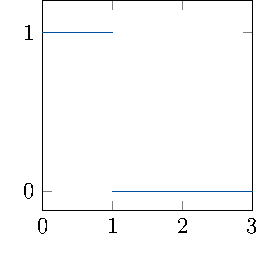
\includegraphics{Bspline_B_3_0}
            \caption{Plot of $B_{3,0}$.}
        \end{subfigure}%
        \hspace*{0.005\textwidth}%
        \begin{subfigure}{0.33\textwidth}
        	\centering
			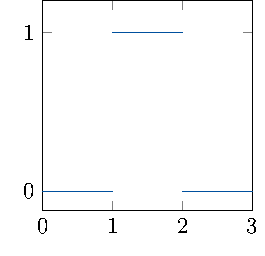
\includegraphics{Bspline_B_4_0}
            \caption{Plot of $B_{4,0}$.}
        \end{subfigure}%
        \hspace*{0.005\textwidth}%
        \begin{subfigure}{0.33\textwidth}
        	\centering
			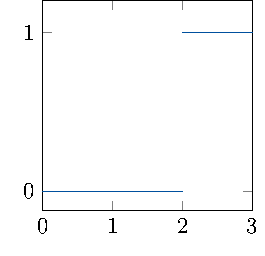
\includegraphics{Bspline_B_6_0}
            \caption{Plot of $B_{6,0}$.}
        \end{subfigure}
        \caption[Plot of B-splines with $\check{p}=0$]{Plot of the non-zero B-splines of order zero, where the knot vector is given by $\Xi = \{0, 0, 0, 1, 2, 2, 3, 3, 3\}$. Note that $B_{j,0}\equiv 0$ for $j\in\{1,2,5,6,7,8\}$.}   
        \label{Fig:Bsplines_p0}   
		\par\bigskip	
		\par\bigskip	
        \begin{subfigure}{0.33\textwidth}
       		\centering
			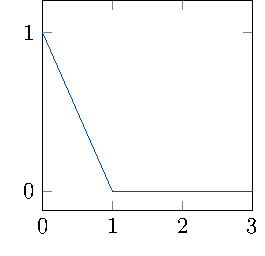
\includegraphics{Bspline_B_2_1}
            \caption{Plot of $B_{2,1}$.}
        \end{subfigure}%
        \hspace*{0.005\textwidth}%
        \begin{subfigure}{0.33\textwidth}
       		\centering
			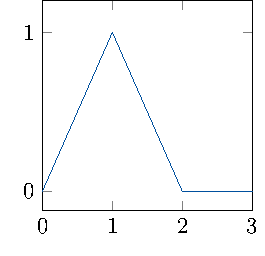
\includegraphics{Bspline_B_3_1}
            \caption{Plot of $B_{3,1}$.}
        \end{subfigure}%
        \hspace*{0.005\textwidth}%
        \begin{subfigure}{0.33\textwidth}
       		\centering
			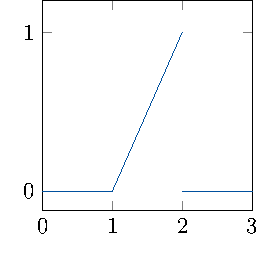
\includegraphics{Bspline_B_4_1}
            \caption{Plot of $B_{4,1}$.}
        \end{subfigure}
		\par\bigskip	
		\par\bigskip	
        \begin{subfigure}{0.33\textwidth}
       		\centering
			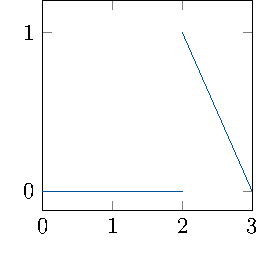
\includegraphics{Bspline_B_5_1}
            \caption{Plot of $B_{5,1}$.}
        \end{subfigure}%
        \hspace*{0.005\textwidth}%
        \begin{subfigure}{0.33\textwidth}
       		\centering
			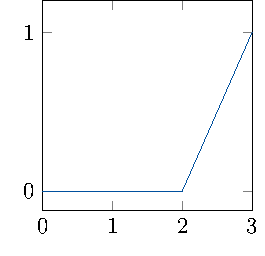
\includegraphics{Bspline_B_6_1}
            \caption{Plot of $B_{6,1}$.}
        \end{subfigure}
        \caption[Plot of B-splines with $\check{p}=1$]{Plot of the non-zero B-spline basis functions (of first degree), where the knot vector is given by $\Xi = \{0, 0, 0, 1, 2, 2, 3, 3, 3\}$. Note that $B_{j,1}\equiv 0$ for $j\in\{1,7\}$.}		
        \label{Fig:Bsplines_p1} 
\end{figure}
\begin{figure}
        \begin{subfigure}{0.33\textwidth}
       		\centering
			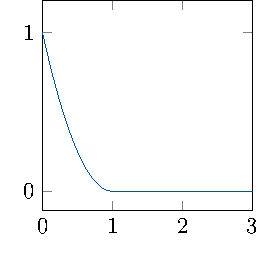
\includegraphics{Bspline_B_1_2}
            \caption{Plot of $B_{1,2}$.}
        \end{subfigure}%
        \hspace*{0.005\textwidth}%
        \begin{subfigure}{0.33\textwidth}
       		\centering
			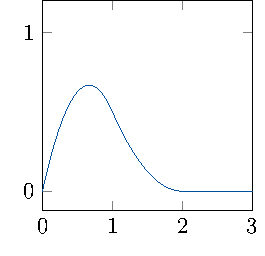
\includegraphics{Bspline_B_2_2}
            \caption{Plot of $B_{2,2}$.}
        \end{subfigure}%
        \hspace*{0.005\textwidth}%
        \begin{subfigure}{0.33\textwidth}
       		\centering
			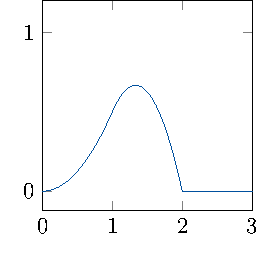
\includegraphics{Bspline_B_3_2}
            \caption{Plot of $B_{3,2}$.}
        \end{subfigure}
		\par\bigskip	
		\par\bigskip	
        \begin{subfigure}{0.33\textwidth}
       		\centering
			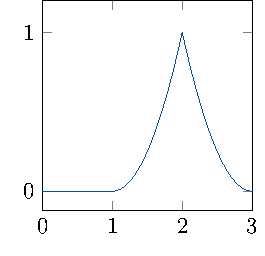
\includegraphics{Bspline_B_4_2}
            \caption{Plot of $B_{4,2}$.}
        \end{subfigure}%
        \hspace*{0.005\textwidth}%
        \begin{subfigure}{0.33\textwidth}
       		\centering
			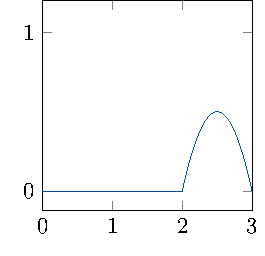
\includegraphics{Bspline_B_5_2}
            \caption{Plot of $B_{5,2}$.}
        \end{subfigure}%
        \hspace*{0.005\textwidth}%
        \begin{subfigure}{0.33\textwidth}
       		\centering
			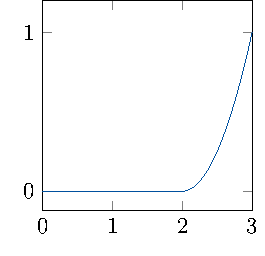
\includegraphics{Bspline_B_6_2}
            \caption{Plot of $B_{6,2}$.}
        \end{subfigure}
        \caption[Plot of B-splines with $\check{p}=2$]{Plot of the 6 different B-spline basis functions (of second degree), where the knot vector is given by $\Xi = \{0, 0, 0, 1, 2, 2, 3, 3, 3\}$.}
        \label{Fig:Bsplines_p2}   
\end{figure}
\begin{figure}
        \centering      
        \begin{subfigure}{0.49\textwidth}
       		\centering
			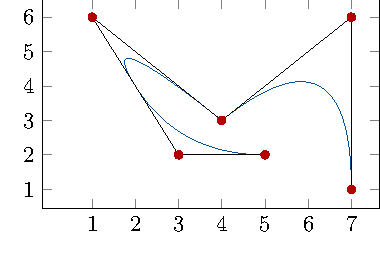
\includegraphics{splineCurve_1}
            \caption{Curve and control polygon.}
        \end{subfigure}%
        \hspace*{0.02\textwidth}%
        \begin{subfigure}{0.49\textwidth}
       		\centering
			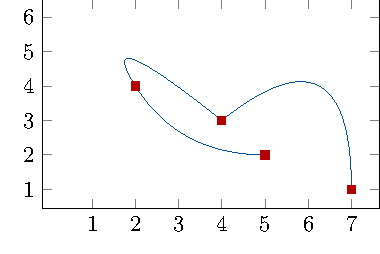
\includegraphics{splineCurve_2}
            \caption{Curve and location of knots.}
        \end{subfigure}
        \caption[Plot of a spline curve]{Plot of a spline curve. Since $\vec{P}_1=(5,2)$, this is the point where the curve starts ($\xi=0$).}\label{Fig:splineCurve}
\end{figure}
By property 7 in the previous list, we see that $B_{1,2}$ and $B_{6,2}$ are discontinuous at $\xi = 0$ and $\xi = 3$, respectively ($\check{p}=2$ and $m=3$ yields $C^{-1}$ continuity in the endpoints). This is characteristic for all open knot vectors. Also note that the repeated knot at $\xi = 2$ forces the function to have the Kronecker delta property; that is, $B_{i,\check{p}}(\xi_j) = \delta_{ij}$ if $\xi_j$ has multiplicity $m=\check{p}$.

We may now define a \textit{spline curve} by
\begin{equation*}
	\vec{P}(\xi) = \sum_{i=1}^n B_{i,\check{p}}(\xi) \vec{P}_i
\end{equation*}
where $\left\{\vec{P}_i\right\}_{i\in[1,n]}$ are the \textit{control points} of the curve. To continue the example, consider the control points $\vec{P}_1=(5,2)$, $\vec{P}_2=(3,2)$, $\vec{P}_3=(1,6)$, $\vec{P}_4=(4,3)$, $\vec{P}_5=(7,6)$ and $\vec{P}_6=(7,1)$. Using the same basis functions $\left\{B_{i,2}\right\}_{i\in[1,6]}$ as in the previous example, we get the curve depicted in \Cref{Fig:splineCurve}. In addition to the curve, the \textit{control polygon} is drawn, which is simply the piece wise linear curve between the ordered control points. Note that the smoothness of the curve degrades at the point $(4,3)$. This is the result of the repeated knot $\xi = 2$ which yields an interpolation effect, such that the control point lies on the curve (which is also the case at the end points).

\subsection{B-spline knot insertion}
\textit{Knot insertion} is a process for which knots are inserted into the knot vector, which would create more basis function without changing the geometry. This is a very important concept as it allows us to enrich the basis and corresponds for this reason to the classical $h$-refinement procedure in FEM (refining the mesh). This is because the knot vector defines the mesh; such that when more knots are inserted, we get a more refined mesh.

The goal is to insert more knots into $\Xi$ without changing the shape of the curve. We shall do this by \textit{B\"{o}hm's method} (cf. \cite{Lyche2008smd}) which does knot insertion by inserting one knot at a time. Let $\tilde{\Xi}$ be the new knot vector after a knot have been inserted into $\Xi$. Let $\{B_{i,\check{p},\Xi}\}_{i\in [1,n]}$ be the old basis (corresponding to $\Xi$) and $\{B_{i,\check{p},\tilde{\Xi}}\}_{i\in [1,n+1]}$ the new basis after a knot has been inserted (note that since $\tilde{\Xi}$ is known, the basis is completely determined). We then want to find the new set of control points $\left\{\tilde{\vec{P}}_i\right\}_{i\in[1,n+1]}$ (here $\tilde{\vec{P}}_i\in\R^d$ where $d$ is the dimension of the space for which the spline curve belongs) such that
\begin{equation*}
	\vec{P}(\xi) = \sum_{i=1}^n B_{i,\check{p},\Xi}(\xi) \vec{P}_i \overset{!}{=} \sum_{i=1}^{n+1} B_{i,\check{p},\tilde{\Xi}}(\xi) \tilde{\vec{P}}_i.
\end{equation*}
This results in a linear system of equation which could be solved by brute force. However, B\"{o}hm method exploits the support property of B-splines to improve efficiency. Assume that the new knot $\tilde{\xi}$ is inserted in the interval $[\xi_j,\xi_{j+1}]$. Then 
\begin{equation*}
	\tilde{\vec{P}}_i = 
	\begin{cases}
		\vec{P}_i, & \text{if } 1\leq i\leq j-\check{p}\\
		\frac{\tilde{\xi}-\xi_i}{\xi_{i+\check{p}}-\xi_i} \vec{P}_i + \frac{\xi_{i+\check{p}} - \tilde{\xi}}{\xi_{i+\check{p}}-\xi_i} \vec{P}_{i-1}, & \text{if } j-\check{p}+1\leq i\leq j\\
		\vec{P}_{i-1}, & \text{if } j+1\leq i\leq n+1.
	\end{cases}
\end{equation*}
Let's continue our example by inserting the knots $\xi = 0.5$ and $\xi = 1.5$ into our knot vector. We then simply use B\"{o}hms method twice to calculate the new control points. The curve with the mesh before and after the knot insertion is depicted in \Cref{Fig:splineCurveRefined}. 
\begin{figure}
        \centering        
        \begin{subfigure}{0.49\textwidth}
       		\centering
			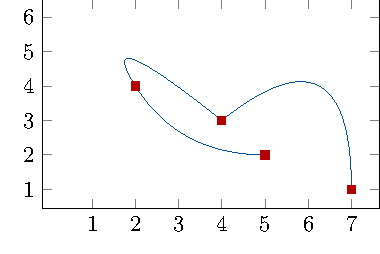
\includegraphics{splineCurve_3}
            \caption{Curve with mesh before refinement.}
        \end{subfigure}%
        \hspace*{0.02\textwidth}%
        \begin{subfigure}{0.49\textwidth}
       		\centering
			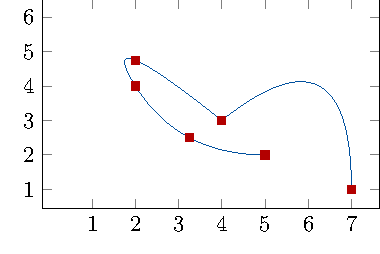
\includegraphics{splineCurve_4}
        	\caption{Curve with mesh after refinement.}
        \end{subfigure}
        \caption{Mesh comparison for knot refinement.}\label{Fig:splineCurveRefined}
\end{figure}
In \Cref{Fig:splineCurveRefined2} we see that the control polygon has changed. Indeed, it has moved towards the curve where the refinement has occurred, which is another nice property of knot insertion.
\begin{figure}
        \centering        
        \begin{subfigure}{0.49\textwidth}
       		\centering
			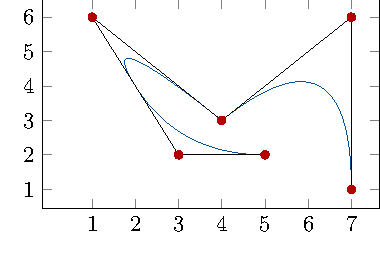
\includegraphics{splineCurve_5}
            \caption{Control polygon before refinement.}
        \end{subfigure}%
        \hspace*{0.02\textwidth}% 
        \begin{subfigure}{0.49\textwidth}
       		\centering
			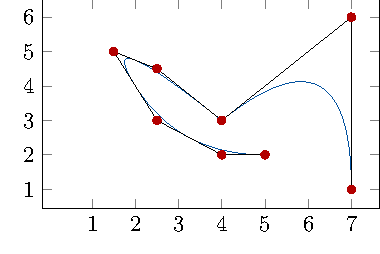
\includegraphics{splineCurve_6}
            \caption{Control polygon after refinement.}
        \end{subfigure}
        \caption{Control polygon comparison for knot insertion.}\label{Fig:splineCurveRefined2}
\end{figure}

\subsection{B-spline degree elevation}
Having a basis of a higher order creates more accurate solution in FEM/IGA. Thus, we want to have an algorithm which increase the order from $\check{p}$ to $\check{p}+m$ without changing the geometry and the parametric space. Since the continuity at each knot must be preserved, it follows from property 7 on page \pageref{List:properties} that we must increase the multiplicity of each knot by $m$. We also need to find the new set of control points. As for knot insertion, we must find the new set of control points $\left\{\vec{Q}_i\right\}_{i\in[1,\tilde{n}]}$ such that
\begin{equation*}
	\vec{P}(\xi) = \sum_{i=1}^n B_{i,\check{p},\Xi}(\xi) \vec{P}_i \overset{!}{=} \sum_{i=1}^{\tilde{n}} B_{i,\check{p}+m,\tilde{\Xi}}(\xi) \vec{Q}_i =: \vec{Q}(\xi).
\end{equation*}
Let $S$ be an integer such that $S+1$ is the number of unique knots in $\Xi$. Since $\Xi$ is open ($\xi_1=\dots=\xi_{\check{p}+1}$ and $\xi_{n+1}=\dots=\xi_{n+\check{p}+1}$), it may be written on the form
\begin{align*}
	\Xi &= \{\underbrace{\xi_1,\dots,\xi_{\check{p}+1}}_{p+1}, \xi_{\check{p}+2},\dots,\xi_n,\underbrace{\xi_{n+1},\dots,\xi_{n+\check{p}+1}}_{\check{p}+1}\}\\
		&= \{\underbrace{u_0,\dots,u_0}_{\check{p}+1},\underbrace{u_1,\dots,u_1}_{z_1},\dots,\underbrace{u_{S-1},\dots,u_{S-1}}_{z_{S-1}},\underbrace{u_S,\dots,u_S}_{\check{p}+1}\}
\end{align*}
where $z_i$ denotes the multiplicity of the knot with value $u_i$ for $i=1,\dots,S-1$. If we now want to elevate the degree $m$ times (from $\check{p}$ to $\check{p}+m$), we get the new knot vector
\begin{align*}
	\tilde{\Xi} &= \{\underbrace{\tilde{\xi}_1,\dots,\tilde{\xi}_{\check{p}+1+m}}_{\check{p}+1+m}, \tilde{\xi}_{\check{p}+2},\dots,\tilde{\xi}_{\tilde{n}},\underbrace{\tilde{\xi}_{\tilde{n}+1},\dots,\tilde{\xi}_{\tilde{n}+\check{p}+1+m}}_{\check{p}+1+m}\}\\
	&= \{\underbrace{u_0,\dots,u_0}_{\check{p}+1+m},\underbrace{u_1,\dots,u_1}_{z_1+m},\dots,\underbrace{u_{S-1},\dots,u_{S-1}}_{z_{S-1}+m},\underbrace{u_S,\dots,u_S}_{\check{p}+1+m}\}.
\end{align*}
It is also easy to observe that the new number of basis functions is given by $\tilde{n}=n+S\cdot m$. What remains to be found is the new set of control points $\left\{\vec{Q}_i\right\}_{i\in[1,\tilde{n}]}$. Several efficient algorithms exist for this purpose, but we shall follow the idea presented by Huang et al. in~\cite{Huang2004ede}. Since the notation of the article does not correspond to the notation presented here, a complete derivation of the algorithm will be presented here. Denote by $\vec{P}^{(l)}$ the $l$'th derivative of the spline curve of degree $\check{p}$ (which will have degree $\check{p}-l$) such that (using an inductive argument and \Cref{Eq:derivBspline})
\begin{equation*}
	\vec{P}^{(j)}(\xi)=\sum_{i=1}^{n-j} B_{i+l,\check{p}-j,\Xi}(\xi) \vec{P}_i^j \quad\text{and}\quad\vec{Q}^{(j)}(\xi)=\sum_{i=1}^{\tilde{n}-j} B_{i+j,\check{p}+m-j,\tilde{\Xi}}(\xi) \vec{Q}_i^j 
\end{equation*}
where the coefficients $\vec{P}_i^j$ are defined recursively by
\begin{equation}\label{Eq:coeffFormula1}
	\vec{P}_i^j = \begin{cases}\frac{\check{p}+1-j}{\xi_{i+\check{p}+1}-\xi_{i+j}}\left(\vec{P}_{i+1}^{j-1}-\vec{P}_i^{j-1}\right) & \text{if } \xi_{i+\check{p}+1} > \xi_{i+j}\\
	\zerovec & \text{if } \xi_{i+\check{p}+1} = \xi_{i+j}\end{cases}
\end{equation}
for $j>0$, starting with $\vec{P}_i^0 = \vec{P}_i$ for $j=0$. Correspondingly we have,
\begin{equation}\label{Eq:coeffFormula2}
	\vec{Q}_i^j = \begin{cases}\frac{\check{p}+m+1-j}{\tilde{\xi}_{i+\check{p}+m+1}-\tilde{\xi}_{i+j}}\left(\vec{Q}_{i+1}^{j-1}-\vec{Q}_i^{j-1}\right) & \text{if } \tilde{\xi}_{i+\check{p}+m+1} > \tilde{\xi}_{i+j}\\
	\zerovec & \text{if } \tilde{\xi}_{i+\check{p}+m+1} = \tilde{\xi}_{i+j}.\end{cases}
\end{equation}
Note that this implies the following useful formula we shall use later
\begin{equation}\label{Eq:coeffFormula6}
	\vec{Q}_{i+1}^{j-1} = \vec{Q}_i^{j-1}+ \frac{\tilde{\xi}_{i+1+\check{p}+m}-\tilde{\xi}_{i+j}}{\check{p}+m+1-j}\vec{Q}_i^j\qquad	\text{if } \tilde{\xi}_{i+\check{p}+m+1} > \tilde{\xi}_{i+j}.
\end{equation}
Since $u_0=\xi_{j+1}=\xi_{j+1+1}=\dots=\xi_{j+1+\check{p}-j}< \xi_{\check{p}+2}$ for $0\leq j\leq p$, property 6 on page \pageref{List:properties} implies that
\begin{equation*}
	B_{i+j,\check{p}-j,\Xi}(u_0) = \delta_{i+j,j+1}.
\end{equation*}
Hence, 
\begin{equation*}
	\vec{P}^{(j)}(u_0)=\sum_{i=1}^{n-j} B_{i+j,\check{p}-j,\Xi}(u_0) \vec{P}_i^j=\sum_{i=1}^{n-j} \delta_{i+j,j+1} \vec{P}_i^j = \vec{P}_1^j.
\end{equation*}
We have a corresponding result for $\vec{Q}^{(j)}$ such that
\begin{equation*}
	\vec{P}^{(j)}(u_0) = \vec{P}_1^j\quad\text{and}\quad\vec{Q}^{(j)}(u_0) = \vec{Q}_1^j.
\end{equation*}
Moreover, $\vec{P}(\xi)$ and $\vec{Q}(\xi)$ have the same geometry and parameterization (that is, ${\vec{P}^{(j)}(\xi)=\vec{Q}^{(j)}(\xi)}$), and we must therefore have
\begin{equation}\label{Eq:coeffFormula3}
	\vec{Q}_1^j = \vec{P}_1^j
\end{equation}
for $0\leq j\leq p$. 

Define
\begin{equation*}
	\beta_i = \sum_{l=1}^i z_l,
\end{equation*}
such that we have $u_i = \xi_{\beta_i+\check{p}+1}$ (the last of the repeated knot). Let $\check{p}+1-z_i\leq j\leq \check{p}$ and $1\leq i\leq S-1$, such that we only consider the case when the degree of $\vec{P}^{(j)}$ satisfy $p-j\leq z_i-1$. Since the knot $u_i$ is repeated $z_i$ times, property 6 on page \pageref{List:properties} now implies that
\begin{equation*}
	B_{\tilde{i},\check{p}-j,\Xi}(u_i) = \delta_{\tilde{i},\beta_i+1+j},
\end{equation*}
such that
\begin{align*}
	\vec{P}^{(j)}(u_i) &= \sum_{\tilde{i}=1}^{n-j} B_{\tilde{i}+j,\check{p}-j,\Xi}(u_i) \vec{P}_{\tilde{i}}^j = \sum_{\tilde{i}=1}^{n-j} \delta_{\tilde{i}+j,\beta_i+1+j} \vec{P}_{\tilde{i}}^j\\
	&= \vec{P}_{\beta_i+1}^j
\end{align*}
for $\check{p}+1-z_i\leq j\leq p$ and $1\leq i\leq S-1$.

We note that $u_i = \tilde{\xi}_{\beta_i+\check{p}+1+m+im}$ and that this knot has multiplicity $z_i+m$ in $\tilde{\Xi}$. Again, we consider the indices $i$ and $j$ to satisfy $\check{p}+1-z_i\leq j\leq \check{p}$ and $1\leq i\leq S-1$, such that we only consider the case when the degree of $\vec{Q}^{(j)}$ satisfy $\check{p}+m-j\leq z_i+m-1$. Using once again property 6 on page \pageref{List:properties} we have
\begin{equation*}
	B_{\tilde{i},\check{p}+m-j,\tilde{\Xi}}(u_i) = \delta_{\tilde{i},\beta_i+1+j},
\end{equation*}
such that
\begin{align*}
	\vec{Q}^{(j)}(u_i) &= \sum_{\tilde{i}=1}^{\tilde{n}-j} B_{\tilde{i}+j,\check{p}+m-j,\tilde{\Xi}}(u_i) \vec{Q}_{\tilde{i}}^j = \sum_{\tilde{i}=1}^{\tilde{n}-j} \delta_{\tilde{i}+j,\beta_i+1+j} \vec{Q}_{\tilde{i}}^j\\
	&= \vec{Q}_{\beta_i+1}^j
\end{align*}
for $\check{p}+1-z_i\leq j\leq \check{p}$ and $1\leq i\leq S-1$. Using the fact that $\vec{P}^{(j)}(\xi)=\vec{Q}^{(j)}(\xi)$, we have obtained the formula
\begin{equation}\label{Eq:coeffFormula4}
	\vec{Q}_{\beta_i+1+im}^j = \vec{P}_{\beta_i+1}^j,\qquad \check{p}+1-z_i\leq j\leq \check{p},\quad 1\leq i\leq S-1.
\end{equation}
Since $\vec{P}(\xi)$ has degree $\check{p}$, its $(\check{p}+1)$'th derivative must be zero, and thus also the $(\check{p}+1)$'th derivative of $\vec{Q}(\xi)$. Using property 4 on page \pageref{List:properties} and letting $\xi\in [u_i,u_{i+1})=[\tilde{\xi}_{\beta_i+p+1+m+i m},\tilde{\xi}_{\beta_i+\check{p}+1+m+i m+1})$, we have
\begin{align*}
	\zerovec &=\vec{P}^{(\check{p}+1)}(\xi) = \vec{Q}^{(\check{p}+1)}(\xi) = \sum_{\tilde{i}=1}^{\tilde{n}-(\check{p}+1)} B_{\tilde{i}+\check{p}+1,m-1,\tilde{\Xi}}(\xi) \vec{Q}_{\tilde{i}}^{\check{p}+1} \\
	&= \sum_{\tilde{i}=\beta_i+1+i m}^{\beta_i+m+i m} B_{\tilde{i}+\check{p}+1,m-1,\tilde{\Xi}}(\xi) \vec{Q}_{\tilde{i}}^{\check{p}+1},
\end{align*}
which implies, that
\begin{equation*}
	\vec{Q}_{\tilde{i}}^{\check{p}+1} = \zerovec,\qquad \beta_i+1+i m \leq \tilde{i} \leq \beta_i+m+i m,
\end{equation*}
for $0\leq i \leq S-1$. Using \Cref{Eq:coeffFormula6} with $j=\check{p}+1$, we therefore have 
\begin{equation*}
	\vec{Q}_{\tilde{i}+1}^{\check{p}} = \vec{Q}_{\tilde{i}}^{\check{p}},\qquad\beta_i+1+i m \leq \tilde{i} \leq \beta_i+m+i m,\quad 0\leq i \leq S-1,
\end{equation*}
or equivalently
\begin{equation}\label{Eq:coeffFormula5}
	\vec{Q}_{\beta_i+1+i m+l}^{\check{p}} = \vec{Q}_{\beta_i+1+i m}^{\check{p}},\qquad 1 \leq l \leq m,\quad 0\leq i \leq S-1. 
\end{equation}
In addition, we see from \Cref{Eq:coeffFormula2} that $\vec{Q}_{\tilde{i}}^{\check{p}}=\zerovec$ whenever $\tilde{\xi}_{\tilde{i}+\check{p}+m+1} = \tilde{\xi}_{\tilde{i}+\check{p}}$. Since the knots $u_{i+1}$ are repeated $z_{i+1}+m$ times in $\tilde{\Xi}$ (starting at $\tilde{\xi}_{\beta_i+1+\check{p}+im+m+1}$) we have
\begin{equation*}
	\vec{Q}_{\beta_i+1+i m+l}^{\check{p}}=\zerovec,\qquad m+1 \leq l \leq m - 1 + z_{i+1},\quad 0\leq i \leq S-1. 
\end{equation*}
It turns out that these points are not needed.

So, in summary, the algorithm does the following steps
\begin{enumerate}
	\item Set $\vec{P}_i^0 = \vec{P}_i$ for $1\leq i\leq n$. 
	\item Compute $\vec{P}_1^j$ for $0 \leq j \leq \check{p}$ and $\vec{P}_{\beta_i+1}^j$ for $\check{p}+1-z_i\leq j\leq p$ and $1\leq i\leq S-1$ using \Cref{Eq:coeffFormula1}.
	\item Compute $\vec{Q}_1^j$ for $0 \leq j \leq \check{p}$ using \Cref{Eq:coeffFormula3} 
	\item Compute $\vec{Q}_{\beta_i+1+im}^j$ for $p+1-z_i\leq j\leq \check{p}$ and $1\leq i\leq S-1$ using \Cref{Eq:coeffFormula4}.
	\item Compute $\vec{Q}_{\beta_i+1+i m+k}^{\check{p}}$ for $1 \leq k \leq m$ and $0\leq i \leq S-1$ using \Cref{Eq:coeffFormula5}. 
	\item Compute the new control points $\vec{Q}_i=\vec{Q}_i^0$ backwards from \Cref{Eq:coeffFormula6}.
\end{enumerate}
This algorithm may be optimized as discussed in~\cite{Huang2004ede} but will not be presented here as the efficiency of this algorithm is not of great importance for this thesis.

\begin{figure}
        \centering        
        \begin{subfigure}{0.49\textwidth}
       		\centering
			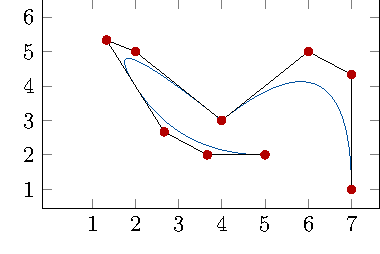
\includegraphics{splineCurve_7}
            \caption{Curve and control polygon after degree elevation.}
            \label{Fig:BsplineCurveDegreeElevated}
        \end{subfigure}%
        \hspace*{0.02\textwidth}%
        \begin{subfigure}{0.49\textwidth}
       		\centering
			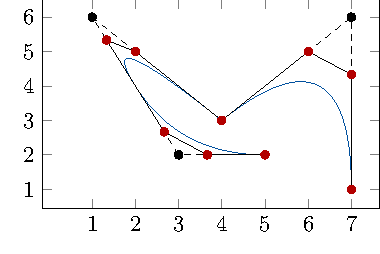
\includegraphics{splineCurve_8}
            \caption{Control polygon comparison showing the corner cutting effect.}
            \label{Fig:BsplineCurveDegreeElevated2}
        \end{subfigure}
        \caption{Control polygon comparison for degree elevation of a spline curve.}
\end{figure}

Continuing our example, let's elevate the degree of the original spline curve by one (from 2 to 3). As we can see in \Cref{Fig:BsplineCurveDegreeElevated}, the geometry of the curve has not changed but the control polygon has changed. As we can see in \Cref{Fig:BsplineCurveDegreeElevated2} only non-interpolating control points in the control polygon have changed. Two new control points replaces each of these control points such that we get a corner cutting effect in the control polygon. Therefore, degree elevation of spline curves is called corner cutting. 

In \Cref{Fig:graphDiffCoeff1} we have a graph which illustrates this process. The points which are colored are used directly to compute coefficients in the set $\{\vec{Q}_i^j\}_{i,j}$ (which have corresponding colors in the graph in \Cref{Fig:graphDiffCoeff2}). Except for $\vec{P}_3^2(0,0)$ (which is set to zero because $\xi_6 = \xi_5$) all points are thus needed.

\begin{figure}
	\centering
	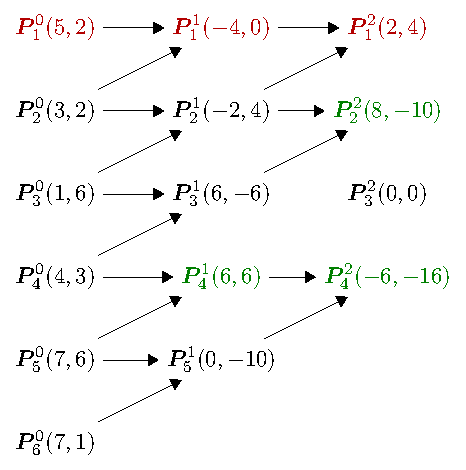
\includegraphics{degreeElevation_1}
	\caption{Graph of differential coefficients of $\vec{P}(\xi)$ in the example.}
	\label{Fig:graphDiffCoeff1}
\end{figure}
In \Cref{Fig:graphDiffCoeff2} we illustrate how the differential coefficients of $\vec{Q}(\xi)$ are computed. The coefficients in red are first computed (step 3), the coefficients in green are then computed (step 4) such that the coefficients in yellow may be computed (step 5). The rest of the coefficients are computed by \Cref{Eq:coeffFormula6}. Note that $\vec{Q}_5^2$ is not really needed.
\begin{figure}
	\centering
	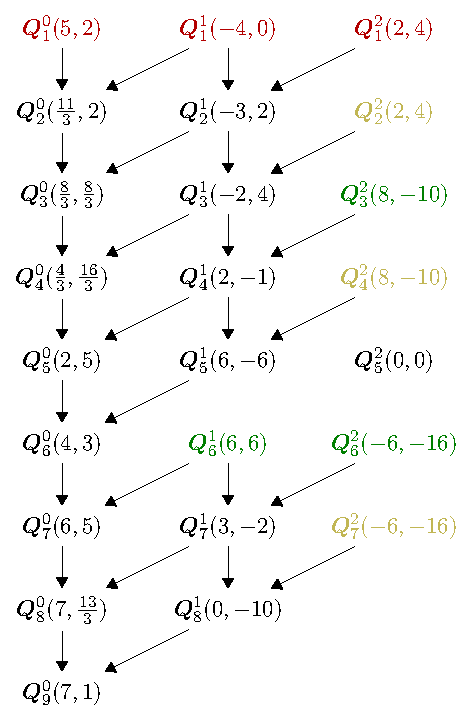
\includegraphics{degreeElevation_2}
	\caption{Differential coefficients of $\vec{Q}(\xi)$ in the example.}
	\label{Fig:graphDiffCoeff2}
\end{figure}
\newpage
\subsection{Spline volumes}
\label{Sec:splineVolumes}
\renewcommand{\Xi}{{\vec{t}_\upxi}}
The extension to bivariate spline surfaces and trivariate spline volumes is straight forward (we shall only here consider volumes). Let $\left\{B_{i,\check{p}_\upxi}\right\}_{i\in[1,n_\upxi]}$, $\left\{B_{j,\check{p}_\upeta}\right\}_{j\in[1,n_\upeta]}$ and $\left\{B_{l,\check{p}_\upzeta}\right\}_{l\in[1,n_\upzeta]}$ be the set of B-spline basis functions in $\xi$-, $\eta$- and $\zeta$-direction, respectively. These sets have their own degree ($\check{p}_\upxi$, $\check{p}_\upeta$ and $\check{p}_\upzeta$, respectively) and knot vectors ($\Xi$, $\Eta$ and $\Zeta$, respectively). A spline volume is then defined by
\begin{equation*}
	\vec{X}(\xi,\eta,\zeta) = \sum_{i=1}^{n_\upxi}\sum_{j=1}^{n_\upeta}\sum_{l=1}^{n_\upzeta} B_{i,\check{p}_\upxi}(\xi)B_{j,\check{p}_\upeta}(\eta)B_{l,\check{p}_\upzeta}(\zeta)\vec{P}_{i,j,l}.
\end{equation*}
We may extend our spline curve example into a volume by adding the knot vectors $\Eta = \{0, 0, 1, 1\}$ and $\Zeta = \{0, 0, 1, 1\}$. By adding appropriate control points, we get the spline volume in \Cref{Fig:SplineVolume}. We have here in addition to the volume drawn the mesh on top showing three elements. 
\begin{figure}
	\centering        
	\begin{subfigure}{0.49\textwidth}
		\centering     
		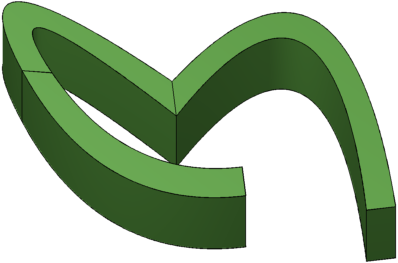
\includegraphics[width=0.7\textwidth]{splineVolume}
		\caption{Spline volume.}
	\end{subfigure}%
    \hspace*{0.02\textwidth}%
	\begin{subfigure}{0.49\textwidth}
		\centering     
		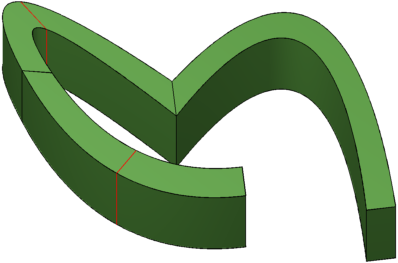
\includegraphics[width=0.7\textwidth]{splineVolumeKnotIns1}
		\caption{Knots inserted in the $\xi$-direction.}
	\end{subfigure}
	\bigskip\par
	\bigskip\par
	\begin{subfigure}{0.49\textwidth}
		\centering     
		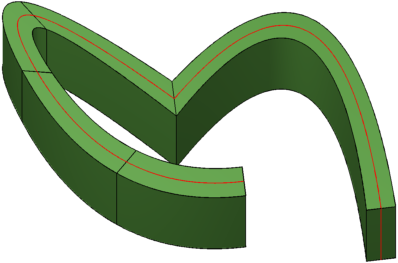
\includegraphics[width=0.7\textwidth]{splineVolumeKnotIns2}
		\caption{Knots inserted in the $\eta$-direction.}
	\end{subfigure}%
    \hspace*{0.02\textwidth}%
	\begin{subfigure}{0.49\textwidth}
		\centering     
		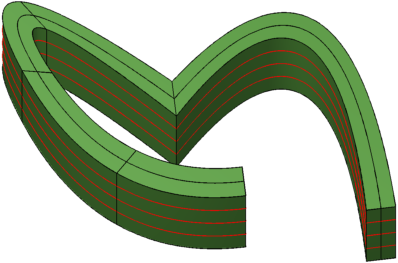
\includegraphics[width=0.7\textwidth]{splineVolumeKnotIns3}
		\caption{Knots inserted in the $\zeta$-direction.}
	\end{subfigure}
	\caption[Spline volume and its knot insertions]{Spline volume and its knot insertions. We here choose to first insert knots in the $\xi$-direction followed by the $\eta$- and $\zeta$-direction, respectively.}
	\label{Fig:SplineVolume}
\end{figure}

Once again, we want to be able to refine this mesh into more elements without changing the geometry. For spline volumes, this is done by refining the mesh in each parameter direction (in the $\xi$-, $\eta$- and $\zeta$-direction). This refining process thus involves refining in each direction separately. For each knot vector, we do knot insertion by B\"{o}hms method once again. Here, we have to order the structure of the control points $\{\vec{P}_{i,j,l}\}$ in a specific way. As an example, say we want to insert $s$ knots in the $\Xi$ direction for a spline object living in a $d$-dimensional space using B\"{o}hms method. We then want to find the new set of control points $\left\{\tilde{\vec{P}}_{i,j,l}\right\}$ such that
\begin{align*}
	\vec{X}(\xi,\eta,\zeta) &= \sum_{i=1}^{n_\upxi}\sum_{j=1}^{n_\upeta}\sum_{l=1}^{n_\upzeta} B_{i,\check{p}_\upxi,\Xi}(\xi)B_{j,\check{p}_\upeta,\Eta}(\eta)B_{l,\check{p}_\upzeta,\Zeta}(\zeta)\vec{P}_{i,j,l}\\
	 &\overset{!}{=} \sum_{i=1}^{n_\upxi+s}\sum_{j=1}^{n_\upeta}\sum_{l=1}^{n_\upzeta} B_{i,p,\tilde{\Xi}}(\xi)B_{j,\check{p}_\upeta,\Eta}(\eta)B_{l,\check{p}_\upzeta,\Zeta}(\zeta)\tilde{\vec{P}}_{i,j,l}.
\end{align*}
We shall use the ordering $\vec{Q}_i = \{\vec{P}_{i,1,1}, \vec{P}_{i,2,1},\dots,\vec{P}_{i,n_\upeta,1},\vec{P}_{i,1,2},\dots,\vec{P}_{i,n_\upeta,n_\upzeta}\}$. We create a new fictitious spline curve given by
\begin{equation*}
	\vec{Q}(\xi) = \sum_{i=1}^{n_\upxi} B_{i,\check{p}_\upxi,\Xi}(\xi) \vec{Q}_i \overset{!}{=} \sum_{i=1}^{n_\upxi+s} B_{i,\check{p}_\upxi,\tilde{\Xi}}(\xi) \tilde{\vec{Q}}_i
\end{equation*}
where $\tilde{\vec{Q}}_i$ is to be determined using B\"{o}hms method $s$ times. Note that this spline curve is in a $(d\cdot n_\upeta\cdot n_\upzeta)$-dimensional space. Reordering $\{\tilde{\vec{Q}}_i\}$ back to the old structure, we obtain the resulting $\{\tilde{\vec{P}}_{i,j,l}\}$. A similar procedure is done if knots are inserted in $\eta$- and $\zeta$-direction. 

Let's say we want to insert the knots $\{0.5, 1.5\}$ in the $\xi$-direction (as we did for the spline curve) and the knots $\{0.5\}$ and $\{0.25, 0.5, 0.75\}$ for the $\eta$- and $\zeta$-direction, respectively. The result (in \Cref{Fig:SplineVolume}) is a refined mesh from 3 elements to 40 elements.

A corresponding procedure is done for degree elevation in spline volumes.

\subsection{NURBS}
\renewcommand{\Xi}{{\vec{t}}}
With the B-splines in our arsenal, we are ready to present Non-Uniform Rational B-Splines (NURBS). Although B-splines may represent many complex curves, there are a class of curves that may not be represented exactly by B-splines, namely, conic sections like circles. Such shapes are often used in engineering, and thus, an extension, which enables this, would be valuable. NURBS enables us to tackle such geometries as well. 

Let $\{w_i\}_{i\in [1,n]}$ be a set of \textit{weights}, and define the \textit{weighting function} by
\begin{equation*}
	W(\xi) = \sum_{\tilde{i}=1}^{n} B_{\tilde{i},\check{p},\Xi}(\xi) w_{\tilde{i}}.
\end{equation*}
The one-dimensional NURBS basis functions can now be defined by
\begin{equation*}
	R_i^{\check{p}}(\xi) = \frac{B_{i,\check{p},\Xi}(\xi)w_i}{W(\xi)},
\end{equation*}
such that a NURBS curve may be expressed by
\begin{equation*}
	\vec{P}(\xi)=\sum_{i=1}^{n} R_i^{\check{p}}(\xi) \vec{P}_i
\end{equation*}
where $\vec{P}_i$ are the control points of the curve.

There are several ways to construct a circle using NURBS (but we need ${\check{p}\geq 2}$). For example, consider the knot vector $\Xi = \{0, 0, 0, \frac14, \frac14, \frac12, \frac12, \frac34, \frac34, 1, 1, 1\}$, the degree $\check{p}=2$, the weights given by $\{w_i\}_{i\in [1,9]}$ where
\begin{equation*}
	w_i = \begin{cases}
		\frac{1}{\sqrt{2}}& \text{for } i \text{ even}\\
		1& \text{otherwise}
	\end{cases}
\end{equation*}
and the control points $\vec{P}_1 = (0,0)$, $\vec{P}_2 = (1,1)$, $\vec{P}_3 = (0,1)$, $\vec{P}_4 = (-1,1)$, $\vec{P}_5 = (-1,0)$, $\vec{P}_6 = (-1,-1)$, $\vec{P}_7 = (0,-1)$, $\vec{P}_8 = (1,-1)$ and $\vec{P}_9 = (1,0)$. This will produce the unit circle, which is depicted in \Cref{Fig:NURBScurve}. Note that there are no non-repeated knots in the knot vector, so we will have interpolation between the location of the knots and the control polygon (since $\check{p} = 2$).
\begin{figure}
	\centering
	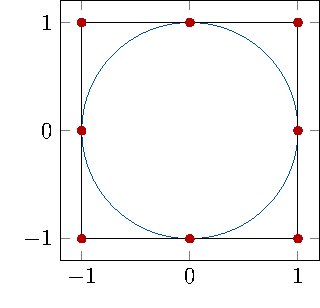
\includegraphics{NURBScurve} 
	\caption[NURBS representation of a unit circle]{NURBS representation of a unit circle with the corresponding control polygon. The curve goes counterclockwise around the unit circle (which is a result of the corresponding ordering in the control points), starts at $(1,0)$ and ends at $(1,0)$.}\label{Fig:NURBScurve}
\end{figure}

\subsection{NURBS knot insertion}
A $d$-dimensional NURBS curve is a projection of a $(d+1)$-dimensional B-spline curve (cf. \cite{Cottrell2009iat}). We may exploit this property to insert new knots into a NURBS. 

Let's say we want to insert $s$ new knots into a NURBS curve defined by the knot vector $\Xi$, the control points $\left\{\vec{P}_i\right\}_{i\in[1,n]}=\left\{(x_i,y_i)\right\}_{i\in[1,n]}$, and the weights $\left\{w_i\right\}_{i\in[1,n]}$. We then construct a 3D B-spline curve with control points given by
\begin{equation*}
	\left\{\vec{Q}_i\right\}_{i\in[1,n]} = \left\{(w_i x_i, w_i y_i, w_i)\right\}_{i\in[1,n]}.
\end{equation*}
We now have a B-spline curve in 3D defined by $\Xi$ (the same knot vector) and the control points $\left\{\vec{Q}_i\right\}_{i\in[1,n]}$. We may now insert knots using B\"{o}hms method as before, which yields the extended knot vector $\tilde{\Xi}$ and the new control points $\left\{\tilde{\vec{Q}}_i\right\}_{i\in[1,n+s]} = \left\{(\tilde{x}_i, \tilde{y}_i, \tilde{w}_i)\right\}_{i\in[1,n+s]}$. Projecting this B-spline curve back to a 2D NURBS with control points given by
\begin{equation*}
	\left\{\tilde{\vec{P}}_i\right\}_{i\in[1,n+s]} = \left\{\left(\frac{\tilde{x}_i}{\tilde{w}_i}, \frac{\tilde{y}_i}{\tilde{w}_i}\right)\right\}_{i\in[1,n+s]}
\end{equation*}
and weights given by $\left\{\tilde{w}_i\right\}_{i\in[1,n+s]}$, we get the refined NURBS. To insert knots in a 3D NURBS curve, we apply an analogous procedure to the control points $\left\{\vec{P}_i\right\}_{i\in[1,n]}=\left\{(x_i,y_i,z_i)\right\}_{i\in[1,n]}$.

In \Cref{Fig:NURBScurveRefined} we have inserted the knots $\{0.5, 0.5, 1.5, 2.25, 2.5, 2.75\}$ into the NURBS circle in \Cref{Fig:NURBScurve}. Note that many of the same properties of B-spline curves are preserved for the NURBS curve. Also note that the mesh is not changed by adding an extra knot at $\xi = 0.5$, but we still have added a new basis function. A reduction of continuity in the basis functions will here occur, but the geometric continuity of the curve remains the same.

\begin{figure}
	\centering    
	\begin{subfigure}{0.49\textwidth}
		\centering
		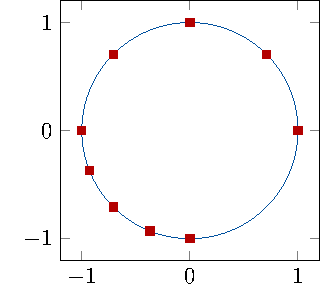
\includegraphics{NURBScurve_2} 
		\caption{Knot locations after refinement.}
	\end{subfigure}%
	\hspace*{0.02\textwidth}%
	\begin{subfigure}{0.49\textwidth}
		\centering
		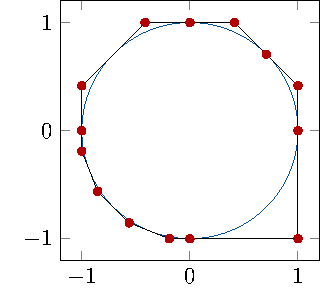
\includegraphics{NURBScurve_3} 
		\caption{Control polygon after refinement.}
	\end{subfigure}      
	\caption{Knot insertion for a NURBS circle.}\label{Fig:NURBScurveRefined}
\end{figure}

\renewcommand{\Xi}{{\vec{t}_\upxi}}
The extensions to bivariate NURBS surfaces and trivariate NURBS volumes are straightforward. For NURBS volumes, let $\left\{B_{i,\check{p}_\upxi,\Xi}\right\}_{i\in[1,n_\upxi]}$, $\left\{B_{j,\check{p}_\upeta,\Eta}\right\}_{j\in[1,n_\upeta]}$ and $\left\{B_{l,\check{p}_\upzeta,\Zeta}\right\}_{k\in[1,n_\upzeta]}$ be the sets of B-spline basis functions in $\xi$-, $\eta$- and $\zeta$-direction, respectively. These sets have their own order ($\check{p}_\upxi$, $\check{p}_\upeta$ and $\check{p}_\upzeta$, respectively) and knot vectors ($\Xi$, $\Eta$ and $\Zeta$, respectively). The trivariate NURBS basis functions are then defined by
\begin{equation}\label{Eq:NURBS3D}
	R_{i,j,l}(\xi,\eta,\zeta) = \frac{B_{i,\check{p}_\upxi,\Xi}(\xi)B_{j,\check{p}_\upeta,\Eta}(\eta)B_{l,\check{p}_\upzeta,\Zeta}(\zeta)w_{i,j,l}}{W(\xi,\eta,\zeta)}
\end{equation}
where the weighting function is now given by
\begin{equation*}
	W(\xi,\eta,\zeta) = \sum_{\tilde{i}=1}^{n_\upxi}\sum_{\tilde{j}=1}^{n_\upeta}\sum_{\tilde{l}=1}^{n_\upzeta}B_{\tilde{i},\check{p}_\upxi,\Xi}(\xi)B_{\tilde{j},\check{p}_\upeta,\Eta}(\eta)B_{\tilde{l},\check{p}_\upzeta,\Zeta}(\zeta)w_{\tilde{i},\tilde{j},\tilde{l}}.
\end{equation*}
In the next section, the single index notation (global indexing system) is used $R_I = R_{i,j,l}$, where for a single patch (with no collapsed control points) we have $I=i+n_\upxi(j-1)+n_\upxi n_\upeta(l-1)$.

The partial derivatives of these functions are then given by the quotient rule. For example, we have
\begin{equation}\label{Eq:NURBS3Dders}
	\frac{\partial R_{i,j,l}}{\partial \xi} = \frac{W(\xi,\eta,\zeta)B_{i,\check{p}_\upxi,\Xi}'(\xi) - W_\xi(\xi,\eta,\zeta)B_{i,\check{p}_\upxi,\Xi}(\xi)}{(W(\xi,\eta,\zeta))^2}B_{j,\check{p}_\upeta,\Eta}(\eta)B_{l,\check{p}_\upzeta,\Zeta}(\zeta)w_{i,j,l}
\end{equation}
where
\begin{equation*}
	W_\xi(\xi,\eta,\zeta) = \sum_{\tilde{i}=1}^{n_\upxi}\sum_{\tilde{j}=1}^{n_\upeta}\sum_{\tilde{l}=1}^{n_\upzeta}B_{\tilde{i},\check{p}_\upxi,\Xi}'(\xi)B_{\tilde{j},\check{p}_\upeta,\Eta}(\eta)B_{\tilde{l},\check{p}_\upzeta,\Zeta}(\zeta)w_{\tilde{i},\tilde{j},\tilde{l}}
\end{equation*}
and
\begin{equation*}
	B_{i,\check{p}_\upxi,\Xi}'(\xi) = \frac{\diff B_{i,\check{p}_\upxi,\Xi}(\xi)}{\diff\xi}.
\end{equation*}
Analogous expressions may be found for the partial derivatives with respect to $\eta$ and $\zeta$.

A 3D NURBS volume is now defined by
\begin{equation*}
	\vec{X}(\xi,\eta,\zeta) = \sum_{i=1}^{n_\upxi}\sum_{j=1}^{n_\upeta}\sum_{l=1}^{n_\upzeta} R_{i,j,l}(\xi,\eta,\zeta)\vec{P}_{i,j,l}
\end{equation*}
Knot insertion into such an object is once again done by inserting knots into a 4D B-splines volume with control points
\begin{equation*}
	\vec{Q}_{i,j,l} = (w_{i,j,l}x_{i,j,l}, w_{i,j,l}y_{i,j,l}, w_{i,j,l}z_{i,j,l}, w_{i,j,l})
\end{equation*}
for $i\in[1,n_\upxi]$, $j\in[1,n_\upeta]$ and $l\in[1,n_\upzeta]$. Using the same procedure as in \Cref{Sec:splineVolumes} we obtain the new set of control points $\tilde{\vec{Q}}_{i,j,l}=(\tilde{x}_{i,j,l}, \tilde{y}_{i,j,l},\tilde{z}_{i,j,l}, w_{i,j,l})$ which after the projection yields our new set of control points for the NURBS volume given by
\begin{equation*}
	\left\{\tilde{\vec{P}}_{i,j,l}\right\}_{i,j,l} = \left\{\left(\frac{\tilde{x}_{i,j,l}}{\tilde{w}_{i,j,l}}, \frac{\tilde{y}_{i,j,l}}{\tilde{w}_{i,j,l}},\frac{\tilde{z}_{i,j,l}}{\tilde{w}_{i,j,l}}\right)\right\}_{i,j,l}
\end{equation*}
and a set of weights given by $\{\tilde{w}_{i,j,l}\}_{i,j,l}$.

A corresponding procedure is done for degree elevation in NURBS volumes.

\subsection{The weak form and Galerkin's method}
The foundation for finite element technologies is the Galerkin's method. Most partial differential equations may not be solved by analytic expressions in closed forms, and one must then resort to numerical methods implemented on some computational resource. As computational resources are limited, the infinitely dimensional function space (in which the solution lies) must be reduced to a finite dimensional function space (where the approximate solution is to be found). Galerkin's method yields the framework for this transition. 

For illustrative purposes, consider the interior Helmholtz equation (in strong form)
\begin{alignat}{3}
	\nabla^2 p + k^2 p &= 0 	\quad &&\text{in}\quad \Omega\subset\R^d,\label{Eq:InteriorHelmholtzEqn}\\
	\partial_n p &= g						&&\text{on}\quad \Gamma=\partial\Omega,\label{Eq:InteriorHelmholtzEqnNeumannCond}
\end{alignat}
where $\partial_n$ denotes the partial derivative in the normal direction, $\vec{n}$, on the surface $\Gamma$ pointing out from the interior domain $\Omega$. Note that this problem is not well posed for certain wave numbers $k$ (corresponding to the eigenfrequencies of the problem).

The \textit{weak form} of the problem is derived from the strong form. Typically, one defines two classes of functions: $\mathcal{S}$ denotes the \textit{solution space} and $\mathcal{V}$ denotes the \textit{test space}. Here, $\mathcal{S}$ is a subspace of the Sobolev space $H^1(\Omega)$ defined by
\begin{equation*}
	H^1(\Omega) = \left\{p\in L^2(\Omega)\st \pderiv{p}{x_i}\in L^2(\Omega),\,\forall i=1,\dots,d\right\}
\end{equation*}
where $L^2(\Omega)$ is the set of square integrable functions. The test space is usually defined to be the same as the solution space, $\mathcal{S} = \mathcal{V}$, which is the Bubnov--Galerkin formulation. When these spaces differ, we have the Petrov--Galerkin formulation which will be investigated in depth in the context of the infinite element method in the second paper.

The Helmholtz equation is first written in weak form. Multiply \eqref{Eq:InteriorHelmholtzEqn} by a test functions $q\in\mathcal{V}$
\begin{equation*}
	q\nabla^2 p + k^2 qp = 0
\end{equation*}
and integrate over $\Omega$
\begin{equation*}
	\int_{\Omega} \left[q\nabla^2 p + k^2 qp\right]\idiff \Omega = 0.
\end{equation*}
Using Greens first identity this can be written as
\begin{equation*}
	-\int_{\Omega} \nabla q\cdot\nabla p\idiff\Omega + \int_{\partial\Omega} q\nabla p\cdot\vec{n}\idiff\Gamma + k^2\int_{\Omega}  qp\idiff \Omega = 0.
\end{equation*}
Thus,
\begin{equation}\label{Eq:weakformulationHelmholtz}
	\int_{\Omega} \nabla q\cdot\nabla p\idiff\Omega -  k^2\int_{\Omega}qp\idiff\Omega = \int_{\partial\Omega} q g\idiff\Gamma.
\end{equation}
The weak formulation then becomes: 
\begin{equation}
	\text{Find} \quad p\in \mathcal{S}\quad\text{such that}\quad B(q,p) = L(q),\qquad \forall q\in \mathcal{V},
\end{equation}
where the bilinear form is given by
\begin{equation}\label{Eq:BilinearForm}
	B(q,p) = \int_{\Omega} \left[\nabla q\cdot\nabla p-  k^2qp\right]\idiff\Omega
\end{equation}
and the corresponding linear form is given by
\begin{equation*}
	L(q) = \int_{\Gamma} qg\idiff\Gamma.
\end{equation*}

We now want to transform this weak statement into a system of algebraic equations. We here apply Galerkin's method and turn to a finite-dimensional subspace $\mathcal{S}_h\subset \mathcal{S}$ (and $\mathcal{V}_h\subset \mathcal{V}$ for the test space). In the IGA context the basis for this subspace is represented by the same splines that parameterizes the domain $\Omega$. The Galerkin approximation of the weak form is now given by:
\begin{equation}\label{Eq:weakformulationHelmholtz_h}
	\text{Find} \quad p_h\in \mathcal{S}_h\quad\text{such that}\quad B(q_h,p_h) = L(q_h),\qquad \forall q_h\in \mathcal{V}_h.
\end{equation}

To find the system of algebraic equations we need to write $p_h$ and $q_h$ as a linear combination of the basis functions (here, the NURBS basis functions, $R_i$)
\begin{equation*}
	q_h = \sum_i R_i c_i\quad\text{and}\quad p_h = \sum_j R_j d_j,
\end{equation*}
respectively. Insertion of these function representations in \Cref{Eq:weakformulationHelmholtz_h} yields
\begin{equation*}
	B\left(\sum_i R_i c_i, \sum_j R_j d_j\right) - L\left(\sum_i R_i c_i\right) = 0
\end{equation*}
which using the bilinearity of $B$ and the linearity of $L$ may be written as
\begin{equation*}
	\sum_i c_i\left(\sum_j B\left(R_i, R_j\right)d_i - L(R_i)\right) = 0.
\end{equation*}
Since the coefficients $c_i$ are arbitrary (the relation should hold for all $q_h\in \mathcal{V}_h$, and in particular $q_h=R_i$ for all $i$) the term in the parentheses must vanish. That is,
\begin{equation*}
	\sum_j B(R_i, R_j)d_j = L(R_i),\quad\forall i.
\end{equation*}
The resulting system of equation may then be written as
\begin{equation*}
	\vec{A}\vec{d}=\vec{F}
\end{equation*}
with components
\begin{align*}
	A_{ij} &= B(R_i, R_j),\\
	F_i &= L(R_i).
\end{align*}
The matrix $\vec{A}$ is usually written as a combination of the \textit{stiffness matrix}, $\vec{K}$ and the \textit{mass matrix}, $\vec{M}$, as $\vec{A} = \vec{K}-k^2\vec{M}$.

\subsection{Assembly}
One typically does not loop through the basis functions. Rather, one loops through the elements constructing local stiffness/mass matrices and successfully place their contribution in the global stiffness/mass matrix. The next step is thus to build the global matrices from the local element matrices, often referred to as assembly.

Let $\Omega^e$ be the domain of a given element, where the index $e$ loops over all elements. The support of the spline basis functions is highly localized. To reduce computations, we should only integrate over functions which have support in $\Omega^e$. Denote by $n_{\mathrm{en}}$ the number of \textit{local shape functions}, $R_a^e$, with support in $\Omega^e$, and let $a$ and $b$ iterate over these functions, we may calculate the entries in the local stiffness matrix as
\begin{equation*}
	k_{ab}^e = \int_{\Omega^e} \nabla R_a^e\cdot\nabla R_b^e \idiff\Omega.
\end{equation*}
Similarly, for the local mass matrix and the local force vector we have
\begin{equation}\label{Eq:loading}
	m_{ab}^e = \int_{\Omega^e} R_a^e R_b^e \idiff\Omega\quad\text{and}\quad f_a^e = \int_{\Gamma^e} R_a^e g\idiff\Gamma,
\end{equation}
respectively. The integration is done by quadrature formulas. One first maps to the parametric domain, and then maps this domain to a parent domain. The element in the parametric domain (corresponding to $\Omega^e$) is given (in 3D) by 
\begin{equation*}
	\hat{\Omega}^e= [\xi_i,\xi_{i+1}]\times[\eta_j,\eta_{j+1}]\times[\zeta_l,\zeta_{l+1}].
\end{equation*}
We want to linearly map this domain into the parent domain $\tilde{\Omega}^e = [-1,1]^d$. So given $(\tilde{\xi},\tilde{\eta},\tilde{\zeta})\in \tilde{\Omega}^e$, we calculate $(\xi,\eta,\zeta)\in \hat{\Omega}^e$ by
\begin{align*}
	\xi &= \xi_i + (\tilde{\xi}+1)\frac{\xi_{i+1}-\xi_i}{2},\\
	\eta &= \eta_j + (\tilde{\eta}+1)\frac{\eta_{j+1}-\eta_j}{2},\\
	\zeta &= \zeta_k + (\tilde{\zeta}+1)\frac{\zeta_{k+1}-\zeta_k}{2}.
\end{align*}
The Jacobian determinant for the parent to parametric mapping is thus given by
\begin{equation*}
	J_2 = \begin{vmatrix}
		\frac{\partial \xi}{\partial\tilde{\xi}} & \frac{\partial \xi}{\partial\tilde{\eta}} & \frac{\partial \xi}{\partial\tilde{\zeta}}\\
		\frac{\partial \eta}{\partial\tilde{\xi}} & \frac{\partial \eta}{\partial\tilde{\eta}} & \frac{\partial \eta}{\partial\tilde{\zeta}}\\
		\frac{\partial \zeta}{\partial\tilde{\xi}} & \frac{\partial \zeta}{\partial\tilde{\eta}} & \frac{\partial \zeta}{\partial\tilde{\zeta}}\\
	\end{vmatrix}=\frac{1}{8}(\xi_{i+1}-\xi_i)(\eta_{j+1}-\eta_j)(\zeta_{k+1}-\zeta_k).
\end{equation*}
Similarly, we need the Jacobian for the mapping from the parametric domain into the physical domain. Given $(\xi,\eta,\zeta)\in \hat{\Omega}^e$, we calculate $\vec{X}\in \Omega^e$ by
\begin{align*}
\vec{X} =
	\begin{bmatrix}
	x_1\\
	x_2\\
	x_3
	\end{bmatrix} = 
	\sum_{i=1}^{n_\upxi}\sum_{j=1}^{n_\upeta}\sum_{l=1}^{n_\upzeta} R_{i,j,l}(\xi,\eta,\zeta) \vec{P}_{i,j,l} = \sum_{a=1}^{n_{\mathrm{en}}} R_a^e(\xi,\eta,\zeta) \vec{P}_a
\end{align*}
where $\vec{P}_{i,j,k}$ are the control points and $R_{i,j,l}^{\check{p}_\upxi,\check{p}_\upeta,\check{p}_\upzeta}$ are the NURBS basis functions which are computed by \Cref{Eq:NURBS3D}. We shall denote this mapping by $\vec{X}: \hat{\Omega} \rightarrow \Omega$. Note that the last equality again comes from the highly localized support of the NURBS basis. The Jacobian matrix is then given by
\begin{equation}\label{Eq:NURBSjacobian}
	\vec{J} = \begin{bmatrix}
		\frac{\partial x_1}{\partial \xi} & \frac{\partial x_1}{\partial \eta} & \frac{\partial x_1}{\partial \zeta}\\
		\frac{\partial x_2}{\partial \xi} & \frac{\partial x_2}{\partial \eta} & \frac{\partial x_2}{\partial \zeta}\\
		\frac{\partial x_3}{\partial \xi} & \frac{\partial x_3}{\partial \eta} & \frac{\partial x_3}{\partial \zeta}
		\end{bmatrix} = \begin{bmatrix}
		\vec{P}_1, & \vec{P}_2, & \cdots, & \vec{P}_{n_{\mathrm{en}}}
		\end{bmatrix}\begin{bmatrix}
			\frac{\partial R_1}{\partial \xi} & \frac{\partial R_1}{\partial \eta} & \frac{\partial R_1}{\partial \zeta}\\
			\frac{\partial R_2}{\partial \xi} & \frac{\partial R_2}{\partial \eta} & \frac{\partial R_2}{\partial \zeta}\\
			\vdots &\vdots &\vdots \\
			\frac{\partial R_{n_{\mathrm{en}}}}{\partial \xi} & \frac{\partial R_{n_{\mathrm{en}}}}{\partial \eta} & \frac{\partial R_{n_{\mathrm{en}}}}{\partial \zeta}\\
		\end{bmatrix}
\end{equation} 
such that the Jacobian determinant of this mapping is given by
\begin{equation*}
	J_1 = \mathrm{det}(\vec{J})
\end{equation*}
where the derivatives of the NURBS basis functions are computed by \Cref{Eq:NURBS3Dders}. The local stiffness matrix contains derivatives of the NURBS functions w.r.t. physical coordinates, and so we need to find expressions for $\frac{\partial R_i}{\partial x_j}$. By the chain rule we have
\begin{align*}
	\frac{\partial R_i}{\partial \xi} &= \frac{\partial R_i}{\partial x_1}\frac{\partial x_1}{\partial \xi} + \frac{\partial R_i}{\partial x_2}\frac{\partial x_2}{\partial \xi} + \frac{\partial R_i}{\partial x_3}\frac{\partial x_3}{\partial \xi}\\
	\frac{\partial R_i}{\partial \eta} &= \frac{\partial R_i}{\partial x_1}\frac{\partial x_1}{\partial \eta} + \frac{\partial R_i}{\partial x_2}\frac{\partial x_2}{\partial \eta} + \frac{\partial R_i}{\partial x_3}\frac{\partial x_3}{\partial \eta}\\
	\frac{\partial R_i}{\partial \zeta} &= \frac{\partial R_i}{\partial x_1}\frac{\partial x_1}{\partial \zeta} + \frac{\partial R_i}{\partial x_2}\frac{\partial x_2}{\partial \zeta} + \frac{\partial R_i}{\partial x_3}\frac{\partial x_3}{\partial \zeta}.
\end{align*}
And thus, we may write
\begin{equation}
	\begin{bmatrix}
		\frac{\partial R_i}{\partial x_1}, & \frac{\partial R_i}{\partial x_2},& \frac{\partial R_i}{\partial x_3}
	\end{bmatrix}\vec{J} = 
	\begin{bmatrix}
		\frac{\partial R_i}{\partial \xi}, & \frac{\partial R_i}{\partial \eta},& \frac{\partial R_i}{\partial \zeta}
	\end{bmatrix}.
\end{equation}
Multiplying with the inverse of the Jacobian, $\vec{J}^{-1}$, from the right, and taking the transpose on each side of the equation finally yields
\begin{equation}\label{Eq:basisFunsDerivativeRel}
	\begin{bmatrix}
		\frac{\partial R_i}{\partial x_1}\\
		\frac{\partial R_i}{\partial x_2}\\
		\frac{\partial R_i}{\partial x_3}
	\end{bmatrix} = 
	\vec{J}^{-\transpose}
	\begin{bmatrix}
		\frac{\partial R_i}{\partial \xi}\\
		\frac{\partial R_i}{\partial \eta}\\
		\frac{\partial R_i}{\partial \zeta}
	\end{bmatrix}.
\end{equation}
With these expressions in mind the local mass matrix can be computed in the parent domain as
\begin{equation*}
	m_{ab}^e = \int_{\tilde{\Omega}^e} R_a^e R_b^e J_1 J_2 \idiff\tilde{\Omega}.
\end{equation*}
Collecting the basis functions $R_a^e$ being non zero on the element, $\Omega^e$, into a vector ${\vec{R}^e =[R_1^e, R_2^e, \dots, R_{n_{\mathrm{en}}}^e]^\transpose}$ enables us to write the full local element mass matrix in terms of an outer product
\begin{equation*}
	\vec{m}^e = \int_{\tilde{\Omega}^e} \vec{R}^e [\vec{R}^e]^\transpose J_1 J_2 \idiff\tilde{\Omega},
\end{equation*}
with corresponding expressions for the local stiffness matrix and the local force vector. 

The integrals are approximated with quadrature rules. If we want to approximate the integral
\begin{equation*}
	\int_{\tilde{\Omega}} g(\tilde{\xi}, \tilde{\eta}, \tilde{\zeta}) \idiff \tilde{\Omega},
\end{equation*}
the approximation by Gaussian quadrature is given by
\begin{equation*}
	\int_{\tilde{\Omega}} g(\tilde{\xi}, \tilde{\eta}, \tilde{\zeta}) \idiff \tilde{\Omega} \approx \sum_{i=1}^{n_{\mathrm{q}}} \rho_i g(\tilde{\xi}_i, \tilde{\eta}_i, \tilde{\zeta}_i),
\end{equation*}
where $n_{\mathrm{q}}$ are the number of quadrature points, and $(\tilde{\xi}_i, \tilde{\eta}_i, \tilde{\zeta}_i)$ and $\rho_i$ are given quadrature points and weights, respectively.

\subsection{Error analysis}
In developing the ASIGA\footnote{The ASIGA (Acoustic Scattering using IsoGeometric Analysis) toolbox is available at the Zetison/ASIGA GitHub repository.} toolbox (developed in \MATLAB) for this PhD the error analysis has been a crucial debugging and researching approach. It is not only crucial to obtain numerical evidence for the correctness of the implemented code, but it can be used in research to compare methods. It is typically done by finding an analytic solution and analyze the convergence of the numerical solution towards this analytic solution in some suitable norm. What norm to compute the error in is not obvious and is very much problem dependent. For V-elliptic problems like the Poisson problem it is natural to use the energy norm defined by the $H^1$-semi norm
\begin{equation*}
	\energyNorm{u}{\Omega} = \sqrt{B(u, u)} = |u|_{H^1}, \quad\text{with}\quad B(v,u) = \int_\Omega \nabla v\cdot\nabla u\idiff \Omega
\end{equation*}
as Galerkin's method minimizes the error in this norm. In~\cite{Johannessen2014iau} we find the following result: Let $\check{p}$ be the highest degree of a complete polynomial in the FE basis and denote by $\|u\|_{H^{\check{p}+1}}$ the Sobolev norm of order $\check{p}+1$. For problems where the solution is not sufficiently smooth, $u\not\in H^{\check{p}+1}$ we have the error bound
\begin{equation*}
	\energyNorm{u - u_h}{\Omega}\leq C h^\alpha\| u\|_{H^{\alpha+1}}
\end{equation*}
where the constant $C$ is among other things dependent of the transformation from the parametric space to the physical space. It is not however depending on the maximal element size\footnote{The element size is defined as the smallest ball in which the element can be inscribed.}, $h$. So as $h$ become smaller, we expect the convergence to be of order $\alpha$ which is defined by
\begin{equation*}
	\alpha = \min\{\check{p},\lambda\}
\end{equation*}
where $\lambda$ is the strength of the singularity. Such that $\lambda<\check{p}$ limits the rate of convergence to the strength of singularity, rather than the polynomial order. This problem may be resolved by using adaptive mesh refinement to obtain $\alpha=\check{p}$. That is, one can obtain the same convergence as for sufficiently smooth solutions $u$. Adaptive mesh refinement (AMR) using T-splines was investigated in~\cite{Bazilevs2010iau,Scott2012lro}. Moreover, the recent LR B-splines was introduced in \cite{dokken2013pso} followed by AMR analysis in \cite{Johannessen2015dcd,Johannessen2015ots,Kumar2015sap,Kumar2017spr}. Other AMR techniques include THB-splines~\cite{Giannelli2012tst,Wei2015thc} and U-splines~\cite{Sangalli2016uss}. As suggested in~\cite{Gerdes1996so3}, the need for AMR applies to solving Helmholtz problems as well. 

The Helmholtz equation (with $B$ defined in~\Cref{Eq:BilinearForm}) is not, however, V-elliptic~\cite[p. 46]{Ihlenburg1998fea}. In fact, $B$ does not even induce a semi-norm. Moreover, for comparison with the boundary element method using volumetric norms is not only unfeasible, but these methods obtain super convergence in appropriate negative fractional Sobolev norms~\cite{Dolz2016aib}. Each method may have a preferred norm in which it excels and a priori error estimates often exist in such cases and it certainly makes sense to use these norms for code development. For research purposes it is not clear in which norm the comparison should be made. In the context of acoustic scattering with the target strength being the quantity of interest, it is natural to consider a norm over the boundary of the scatterer, $\Gamma$, since the far field is computed based on the Helmholtz integral (\Cref{Eq:HelmholtzIntegralFarField}) over the same domain. The $L^2(\Gamma)$-norm then represent an arguably good compromise in this context and has been used frequently in this thesis.







